\section{Summary of contributions}

This thesis makes several significant contributions to the study of diagramming, diagramming tools, and educational technology, including:

\begin{itemize}

    \item An interview study of the diagramming process, providing detailed insights into how experts across different domains create and use conceptual diagrams. This study documents how expert from a diverse set of domains author diagrams and identifies key challenges in existing diagramming tools (\cref{chp:interviews}).

    \item A natural diagramming framework that specifies four dimensions of diagramming tool design opportunity that seamlessly and naturally translate diagrammers’ high-level ideas to illustrative and effective diagrams (\cref{sec:natural-diagramming}).
    
    \item \Penrose, a novel system for creating diagrams from plain-text descriptions (\cref{chp:penrose}). \Penrose allows authors to encode domain-specific visual representations and automatically lays out diagrams, bridging the gap between abstract ideas and their visual representation.
    
    \item \Edgeworth, a tool built atop \Penrose, aimed at automating the generation of multiple-choice diagrammatic translation problems (\cref{chp:edgeworth}). 
    
    \item A dataset of translation problems that includes real-world diagrammatic problems in graph theory, chemistry, and Euclidean geometry (\cref{sec:edgeworth-case-studies}).
    
    \item Empirical evidence supporting the reliability, efficiency, and ecological validity of \Edgeworth in educational contexts (\cref{chp:edgeworth-eval}). 
    
\end{itemize}


\section{Future work}

We now discuss potential future directions for \Penrose, \Edgeworth, and diagramming tool research in general. 

\subsection{Composable visual representations}

Over the years of building diagrams using \Penrose and \Edgeworth, we have observed that visual representations in different domains often share common visual components and layout patterns. Further, common visual techniques are widely used in diagramming to convey domain-independent concepts, such as using varying opacity or line weight to highlight parts of a diagram, maintaining layout consistency across multiple diagrams to form a visual narrative, or using sliders or other widgets to drive real-time physical simulations in interactive webpages. It seems natural to separate out these common patterns into their own components, suggesting that \Penrose's existing reusability of visual representations in \Style{} does not provide sufficient flexibility for the needs of digital diagrammers.

In the current version of \Penrose{}, authors can reuse geometric and layout primitives to create new \Style{} programs, and users consume these programs by writing different \Substance{} programs with them. Each \Style{} program is standalone and self-contained, meaning that everything from the styling of points to the color palettes must be defined within that program. In practice, this means that common visual design patterns are copied and pasted between \Style{} files. Additionally, it is common for individual diagrams within a domain to have customized visual elements to draw focus or illustrate a concept. Currently, the only way to override the domain-wide visual style in \Penrose{} is by using workarounds that involve more copying/pasting code in \Style{}. These two limitations result in repetitive and lengthy programs that require high effort to edit and maintain, even for expert \Penrose{} users.

While code duplication and multiple versions of \Style{} may be manageable on a small scale, we envision building a broader ecosystem of diagrams and this requires more flexible reuse mechanisms. We suggest \textbf{composability} as the main design goal for improving \Penrose{}. The existing layout primitives are an example of composability: authors can reuse and \emph{combine} multiple primitives to form new layout problems. Looking forward, we plan to allow diagrammers to create \emph{modules} of visual components and layout patterns. Through this mechanism, an author can draw together multiple different modules they need for their own diagram. And these modules can themselves be composed from other modules: for instance, a module for visualizing complex analysis might make use of lower-level modules for visualizing a coordinate plane and plotting curves, but build on top of that with domain-specific visuals for singularities in holomorphic functions. In addition to user-defined modules, there are also opportunities to build domain-independent visual techniques, such as individual object-level highlighting or annotations, into our languages or as standard library modules.

We believe this composable approach will open up new possibilities for diagrammers to collaborate and create more flexible, reusable, and expressive visual representations. Going forward, we plan to survey existing compose mechanisms such as modules, type systems, and package ecosystems to inform our design for \Penrose.

% leverage research on common building blocks of and layout patterns in specific domains of diagramming, to construct a substrate for composable visual representations.

\subsection{Knowledge-infused problem variation}


% \begin{figure}[h]
%     \centering
%     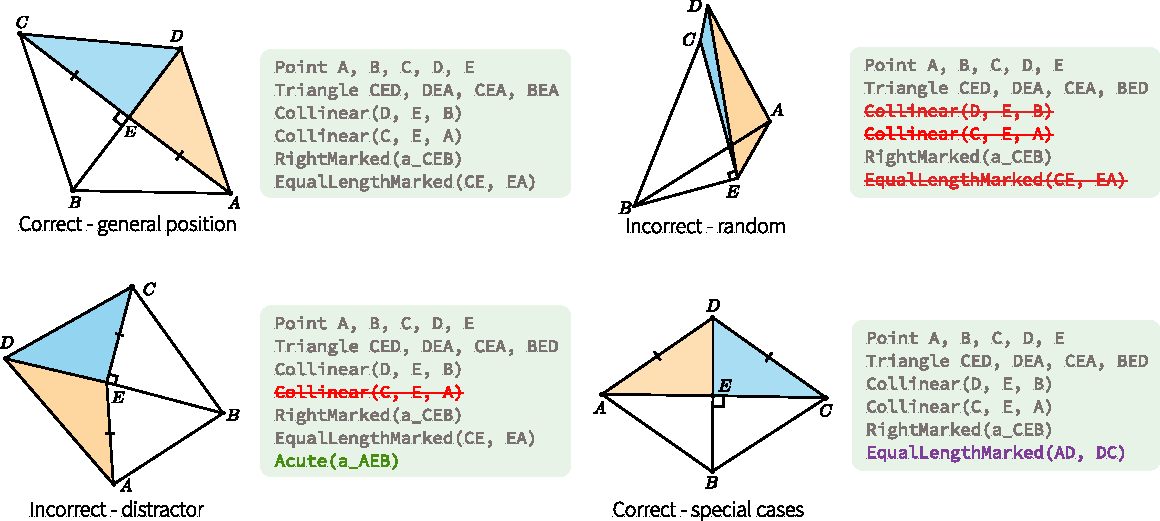
\includegraphics[width=\linewidth]{assets/chapter-3/answer-types.pdf}
%     \caption{Four example classes of problem options. \textbf{Top-left}: the example scenario, representing a general example. \textbf{Bottom-Left}: a counterexample that only slightly differs from the example scenario semantically. \textbf{Top-right}: a counterexample that differs significantly from the prompt. \textbf{Bottom-right}: an example instance that's a corner-case of the prompt.}
%     \label{fig:answer-types}
% \end{figure}

\Edgeworth provides a mixed-initiative~\cite{allen1999mixedinitiative} workflow: authors focus on specifying the content and the general direction of variations through the example scenario, while \Edgeworth fully automates the details of variation generation and layout. The evaluation studies presented in \cref{chp:edgeworth-eval} showed that this workflow improves authoring speed and can produce useful diagrams to educators already. In this section, we focus on the current state of \Edgeworth's outputs and propose future work for improving problem quality.

As discussed in \cref{sec:expert-feedback}, experts used terms like \quotei{obviously incorrect} (E6) and \quotei{less obvious} (E1) to characterize the quality of problem options in a multiple-choice translation problem. Based on their feedback, we divide these options into four categories: given a set of mathematical statements describing logical entities and their relationships, a diagram can be associated with them in one of the following ways:

\vspace{0.5em}
\begin{figure}[h]
\begin{minipage}[b]{0.48\linewidth}
$\bullet$ \textbf{Example}: the diagram represents the math statements, \ie all the statements hold true in the diagram. 
    \vspace{3pt}
    
$\bullet$ \textbf{Counterexample}: the diagram clearly violates the math statements, \ie one or more statements are false in the diagram.
    \vspace{3pt}
    
$\bullet$ \textbf{Positive edge case}: the diagram is an example of the math statements, but contains extraneous entities and/or more specialized relationships. 
    \vspace{3pt}
    
$\bullet$ \textbf{Negative edge case}: the diagram is a counterexample, but only requires a few changes to become an example.
\end{minipage}
\hfill
\begin{minipage}[b]{0.45\linewidth}
    \centering
    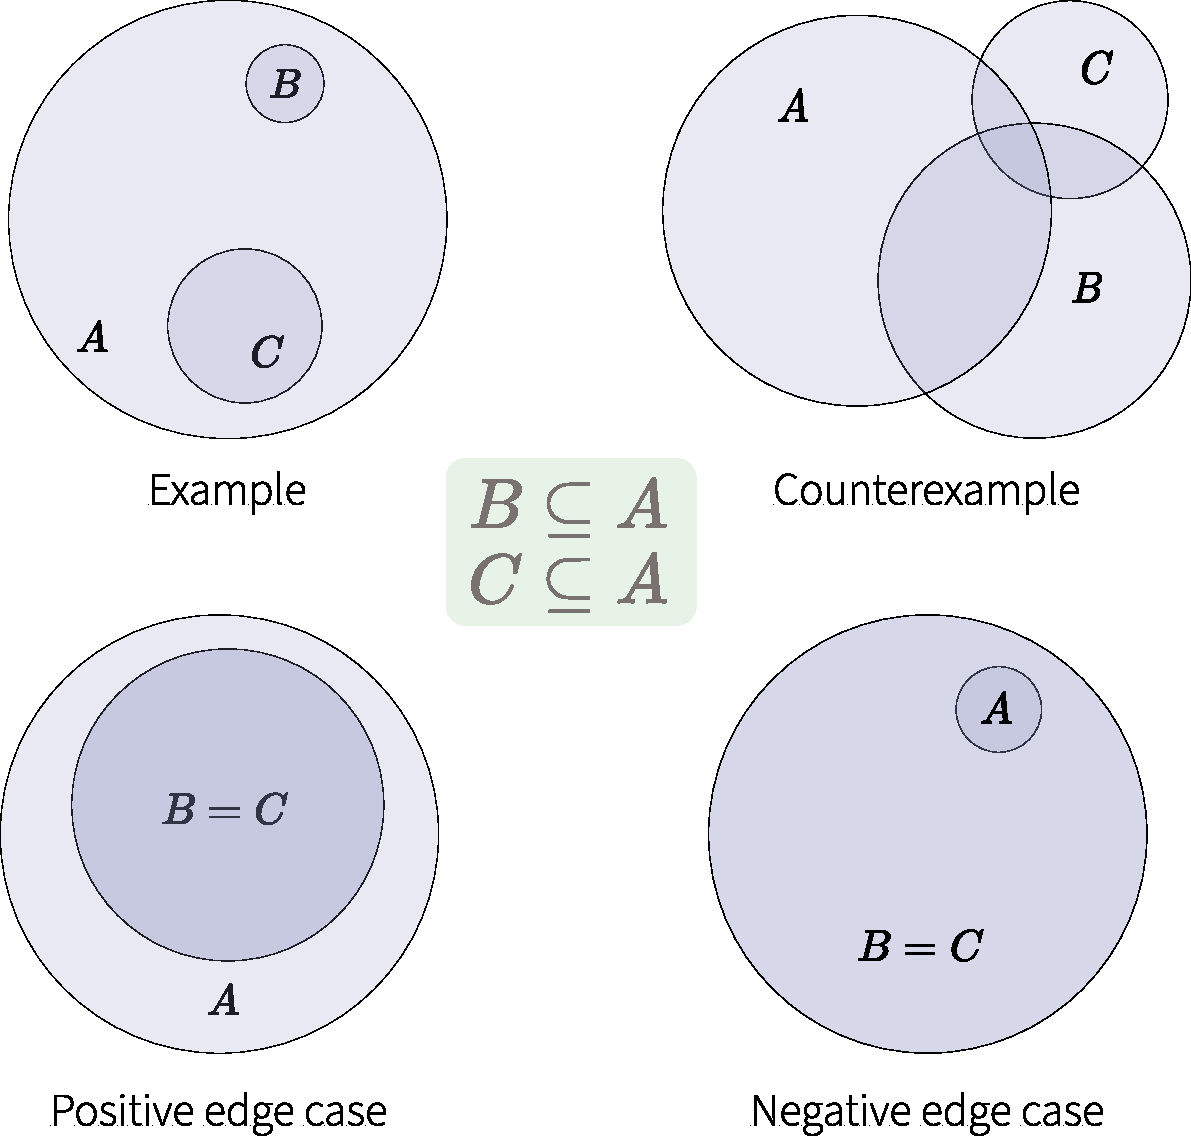
\includegraphics[width=\textwidth]{assets/appendix/definitions-examples.pdf}
\end{minipage}
\end{figure}

\begin{figure}
    \centering
    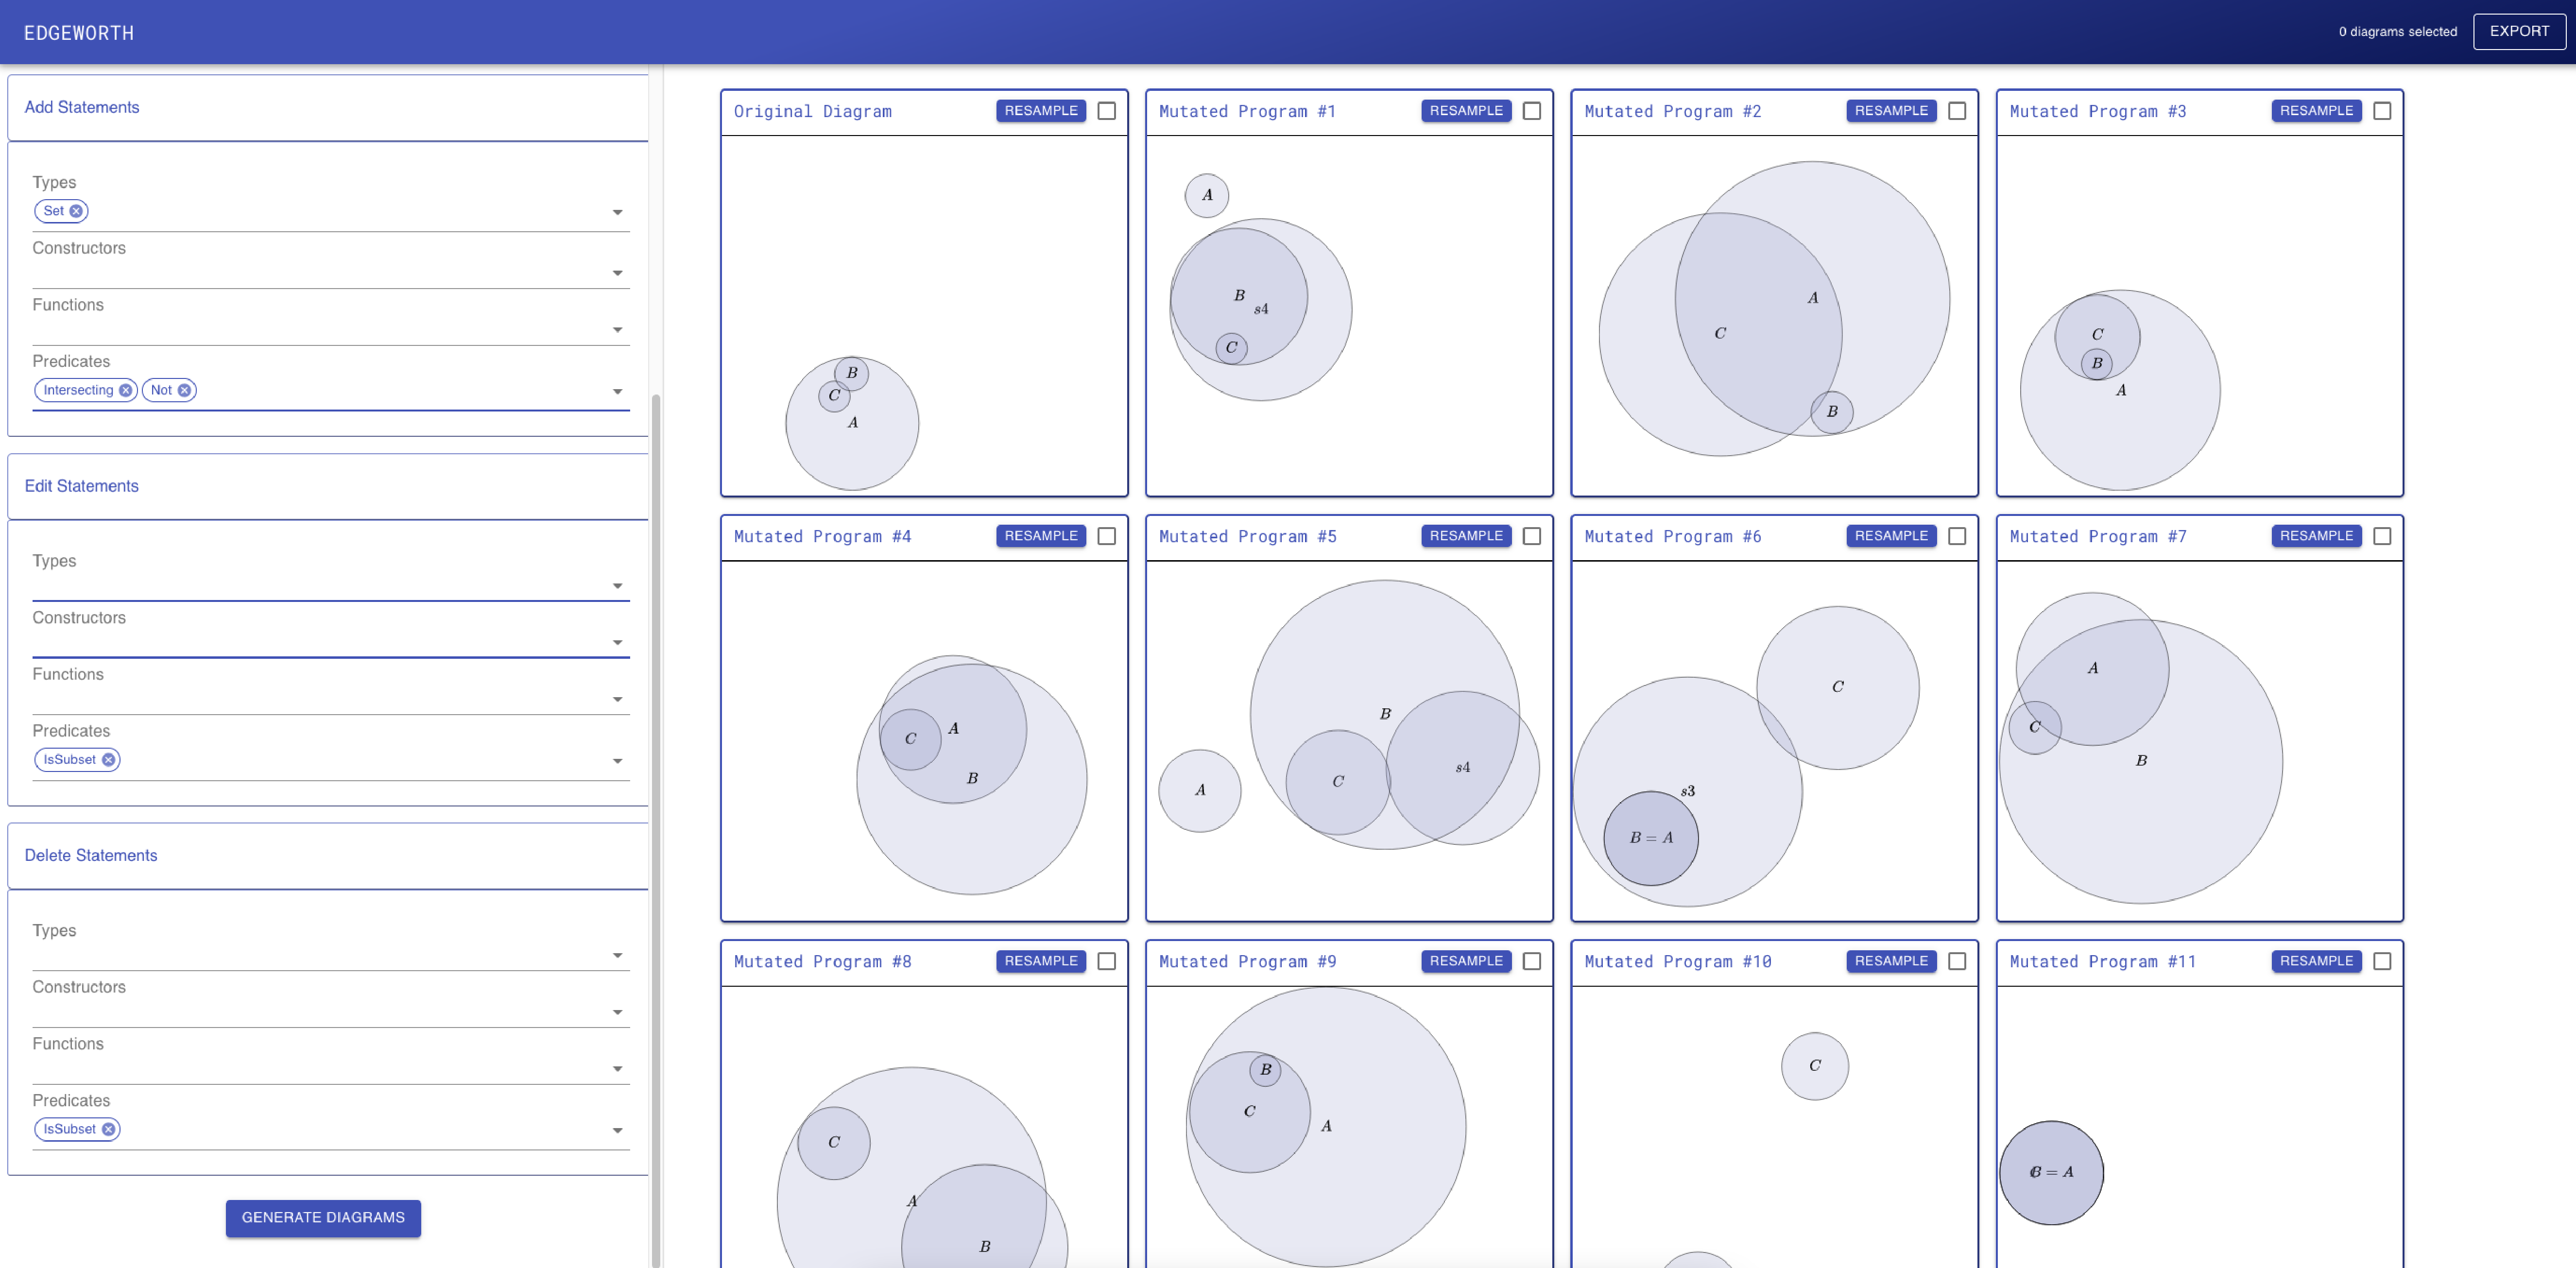
\includegraphics[width=\linewidth]{assets/appendix/edgeworth-bad-output.pdf}
    \caption{A screenshot of the \Edgeworth interface, after generating examples for a translation problem focusing on improper subsets. The first pool of mutants isn't suitable for this problem.}
    \label{fig:edgeworth-bad-output}
\end{figure}

Using \Edgeworth, the author creates an example scenario and \Edgeworth's mutator generates a set of diagrams. When these diagrams don't satisfy the needs of the author (\eg missing counterexamples that are important for an educational goal), the author can only generate more variations and hope to get better ones. For example, suppose an author would like to create problems that test students' knowledge of improper subsets, especially the fact that if $A \subseteq B$, $A = B$ is allowed. Using the \Edgeworth, the author first creates a \Substance program and clicks ``Generate Diagrams.'' 

\noindent\hspace*{\fill}
\begin{minipage}[c]{0.23\columnwidth}
\begin{mdframed}[style=SUBCode]
\begin{lstlisting}[language=Sub-SET,escapechar=@,numbers=none]
Set A, B, C
IsSubset(B, A)
IsSubset(C, A)
\end{lstlisting}
\end{mdframed}
\end{minipage}
\hspace*{\fill}

Ideally, \Edgeworth should generate a set of examples of the subset relations that include the edge cases of $A = B$, $A = C$, or $B = C$, and counterexamples of $B \not\subseteq A$ or $C \not\subseteq A$. However, those particular mutated programs are extremely unlikely to be generated by \Edgeworth. The default \Edgeworth output for this scenario is show in  \cref{fig:edgeworth-bad-output}. There are useful counterexamples, but none of the diagrams include edge cases such as:

\noindent\hspace*{\fill}
\begin{minipage}[c]{0.23\columnwidth}
\begin{mdframed}[style=SUBCode]
\begin{lstlisting}[language=Sub-SET,escapechar=@,numbers=none]
Set A, B, C
IsSubset(B, A)
IsSubset(C, A)
Equal(B, C)
\end{lstlisting}
\end{mdframed}
\end{minipage}
\hspace*{\fill}

\noindent In our experience, it is not uncommon for\Edgeworth to miss important edge cases. 

In future work, we propose to work with Large Language Models (LLMs) to generate high-quality edge cases. Since LLMs are trained on the text of the entire internet, they may contain enough knowledge to suggest pedagogically usefual positive and negative edge cases.

To turn these conceptual edge cases into diagrams, \Penrose{} needs \Substance programs. Therefore, we will first test LLMs capability to generate  \Substance programs.

Consider the case of a teacher authoring the example scenario (\cref{sec:create-scenario}): imagine the teacher specifying the diagram in natural language and an augmented version of \Edgeworth will prompt an LLM to generate the example diagram in \Substance. In preliminary work, we tested this use case and showed that GPT-4 does not do a good job of generating low-level visual code like SVG~\cite{penrosellm}. In contrast, when prompted carefully, GPT-4 can generate \Substance programs which yield correct and legible diagrams.

Assuming reliable \Substance generation capability, an LLM may use the author's inputs (\ie example scenario \Substance and diagram and diagram choices in the mutant pool) together with its embedded domain knowledge to generate pedagogically useful edge cases. \Edgeworth may use a mix of the existing mutation algorithm (\cref{sec:edgeworth-mutation}) and an LLM to generate \Substance programs, for a balance of examples/counterexamples and edge cases. To iterate on the mutant pool, the author picks multiple diagrams in the pool and the LLM can be prompted again with the author's choices in its context to future generate more diagrams based on the author's need.

We note a few challenges with the aforementioned approach. First, LLMs may need help on generating \Substance code because \Substance programs are few in number comparing with other languages in LLMs' training set. In addition to prompt-engineering, future work can experiment with LLM \textit{agents}~\cite{wu_agentkit_2024} so that authors can provide more granular input and feedback to the model. Second, code and natural language may be insufficient to produce high-quality problems, and future work should try leveraging the visual output of \Edgeworth. The recent rise of visual question-answering (VQA) datasets and benchmarks shows a growing interest in improving LLMs visual reasoning capabilities~\cite{lu_mathvista_2024,belouadi_automatikz_2024,fatemi_talk_2023,masry_chartqa_2022}.  While LLMs' ability to reason with just images is still unclear~\cite{rahmanzadehgervi_vision_2024}, all diagrams produced using \Edgeworth have both symbolic (\ie \Substance, \Style, and \Domain) and visual (\ie the output SVGs) representations. Future research should investigate how to incorporate both representations in prompting, fine-tuning, and potentially pre-training of LLMs so that models will be capable of producing high-quality diagrams for all desirable diagram classes.

% In the formative interviews for \Edgeworth (\cref{sec:edgeworth-formative}), we found that the educators we interviewed echoed Kay's concerns~(\cref{sec:edgeworth-formative}). Notably, educators spend significant effort crafting visual learning materials that suit their needs in the classroom. We believe this effort means much more than copy-pasting and low-level tweaking of shapes in a diagram. Instead, educators encode their teaching context and their expertise in this process. Computational tools should provide enough support to provide better ergonomics for the authoring and adaptation of visual learning materials. As our first step, we built \Edgeworth to let educators use one example diagram as the leverage to generate variations of diagrammatic multiple choice problems. There are ample opportunities to use \Edgeworth to create \textit{problem variations}, too. By simply increasing the number of variations and/or using a variation as a new example diagram, the author can use \Edgeworth to generate diagrams for related problems on the same topic. 

% Additionally, experts also expressed interests in using open-ended problems, but also noted that these open-ended problems scaled poorly in practice. In contrast to open-ended problems, automated systems that generate multiple-choice problems are easier to scale up and deliver better learning outcomes for more students if used effectively~\cite{Wang2021}. In this dissertation, we explored how to use \Edgeworth to author a single problem on a particular topic. However, there are ample opportunities to use \Edgeworth to create \textit{problem variations}, too. For instance, \Edgeworth can reliably generate a problem's worth of diagrams within few mutants. The author can also generate problem variations on the same topic by simply increasing the number of mutants. In addition, some \Edgeworth mutants might involve knowledge components that are suitable for problems on another topic. In this case, the author may use the mutant as the example scenario, and run \Edgeworth again to generate diagram variations on that mutant. Future work should study how \Edgeworth can be used in instructional contexts of larger scale.

% AI: the variations we get from \Edgeworth are limited. THere are no knowledge involved in \Edgeworth. Useless variations from \Edgeworth. Large search space. 
% \Edgeworth is both a product of existing AI techniques and a promising platform to assess both domain-specific and general-purpose AI technologies in visual practice authoring. Like many classical AI systems, \Edgeworth makes use of a symbolic description language (\cref{sec:edgeworth-layout}) and mutates the description of the example diagram to search for viable variations. The description language then generates layout constraints that compile to energy functions, the gradients of which drive an optimizer to arrange the diagram layout. In the educational setting, 

% \Edgeworth provides a mixed-initiative~\cite{allen1999mixedinitiative} experience: authors focus on specifying the content and the general direction of variations, while \Edgeworth fully automates the details of variation generation and layout. 

\subsection{Interactive diagrams}


Diagrams live in the context of surrounding text, overlaid annotations, and human gestures. The web opens up opportunities for even richer in-context interaction. In education, though students spend more time on digital platforms, they often see diagrams that are presented exactly as before: pixelated, static, and ornamental. In contrast with a static diagram, a semantics-preserving interactive diagram allows students to rapidly explore alternatives, understand the underlying rules of a visual representation, and receive instant feedback on their actions~\cite{koedinger_learning_2015}. Meaningful interaction with diagrams helps students move from passive recognition to active synthesis of visual representations~\cite{bloomRevised}.

Sadly, interactive diagrams are scarce in the wild. Most interactive documents require authors to be proficient in general-purpose programming and have decent knowledge in handling low-level events like mouse down/up, hover, etc. As a result, a simple interactive diagram often takes up 100s of lines-of-code and can be hard to debug~\cite{callbackSpaghetti, letondal_usability_2010}. Additionally, because interactive diagrams change a lot, authors often need to reason about a collection of diagrams, making the task even harder.

\Penrose and \Edgeworth elevate the semantics of diagrams from low-level primitives to mathematically meaningful notations. Specifically, \Penrose encodes both the translational semantics of how notations are translated to diagrams, and the visual semantics of how shape primitives relate to each other expressed as constraints. By exploiting both, we can automatically support semantics-preserving interactive diagrams. One promising direction of future work is to investigate how to build interactive diagram activities that are automatically derived from \Penrose diagrams without extensive programming effort. In short, I propose to (1) simplify programming interactive diagrams and (2) provide students with rich, automated feedback by leveraging the encoding of visual representations. 

% \section{Motivating example}
% \label{sec:ipenrose-example}

% Consider the first diagram in a popular explorable explanation piece ''Eigenvectors and Eigenvalues Explained Visually~\footnote{\url{https://setosa.io/ev/eigenvectors-and-eigenvalues/}}.''  The diagram is one of a series of interactive diagrams showing the visual properties of eigenvalues and eigenvectors: it shows a visual interpretation of matrices as linear transformations: matrix $A$ with columns $a_1$ and $a_2$ transforms $v$ to $Av$. In the diagram, $a_1$, $a_2$ and $v$ are all draggable. 

% \begin{figure}[h]
%     \centering
%     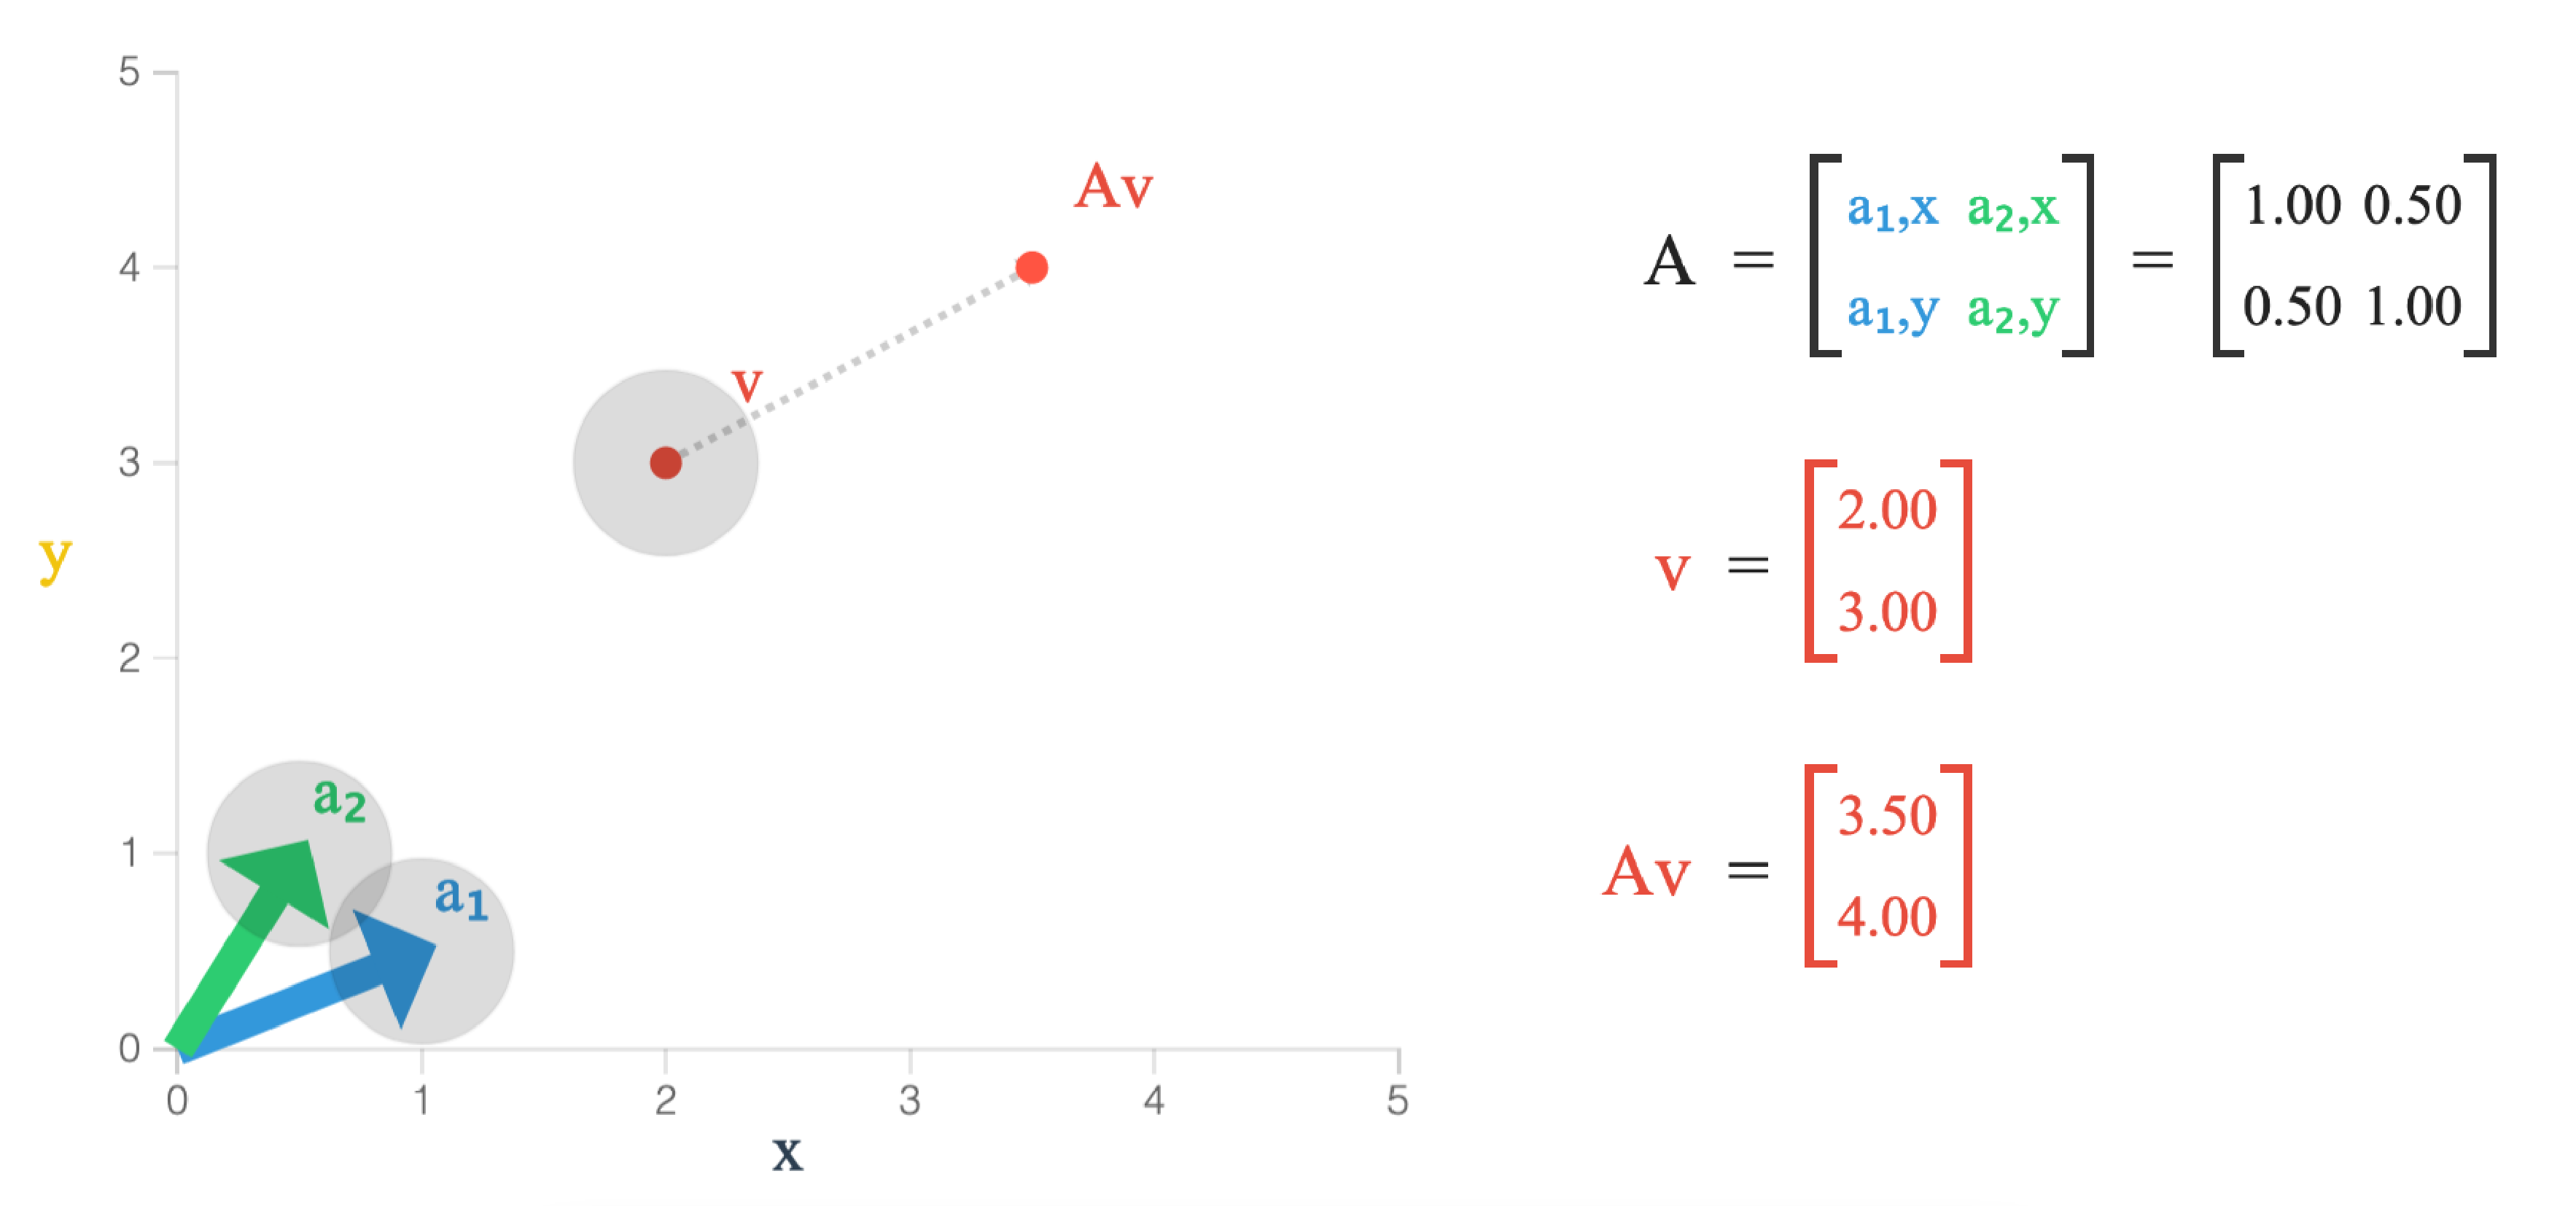
\includegraphics[width=0.8\linewidth]{assets/chapter-4/eigen-visually.pdf}
% \end{figure}

% Seeing what varies and what doesn't is an important form of \emph{feedback} that fosters conceptual understanding. The reader gains an initial understanding of how columns of $A$ impact $Av$’s value through interacting with the diagram: dragging any of $a_1$, $a_2$ and $v$ affects the position of $Av$. 

% In the original code repository~\footnote{\url{https://github.com/vicapow/explained-visually/tree/master/client/explanations/eigenvectors-and-eigenvalues}}, the authors wrote about a hundred lines of JavaScript with D3.js to make the first diagram. Although D3.js and Angular already provide significant support, it's still a lot of work to handle mouse down/up/hover events, and to keep track of intermediate values during dragging. 

% To reproduce this diagram in \Penrose, one can write a simple \Substance program in the linear algebra domain~\cite[Section 5.4]{penrose}. 

% \begin{figure}[h]
%     \centering
%     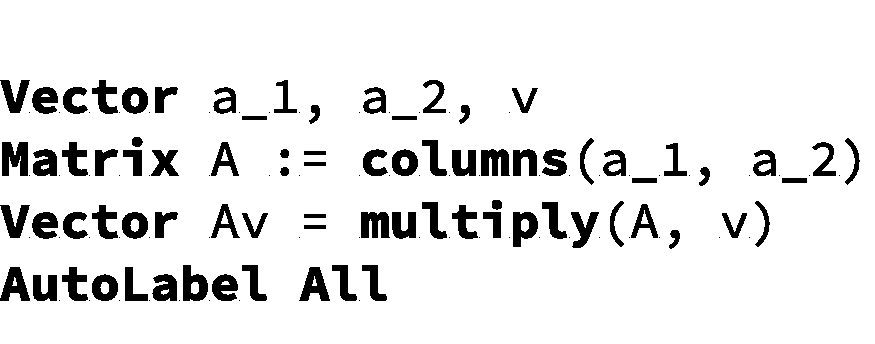
\includegraphics[width=0.4\linewidth]{assets/chapter-4/eigen-substance.pdf}
% \end{figure}

% With the core system, the trio generates a static SVG diagram. Under the hood, every \sub{Vector} is represented visually as an arrow starting at the origin ($a_1$, $a_2$), or a single point ($v$). They are all degrees of freedom (DOF) in the optimization problem. In other words, both the x and y-components of the arrow-end of  $a_1$, $a_2$, and the point representing $v$ are free to move on the canvas. Following the original design of the explorable, the system surfaces the DOFs as draggable points. Whenever the user drags the end of one of the arrows, the optimizer takes the new position as a part of the final solution, and solves the rest of the optimization problem. Effectively, by using this simple and generalizable strategy, which I will discuss in the following sections, the system can reproduce the interactive design using the \Penrose trio for a static diagram \emph{without a single line of code added}.

% \section{Semantics-preserving interactivity as feedback}
% \label{sec:semantic-drag}

% \begin{proposed}
% \cref{sec:ipenrose-example} is an example of a set of interactive behaviors that can be automatically derived from a \Penrose trio without any additional programming.  Specifically, the example leverages how \Penrose encodes visual semantics: \Penrose compiles a program trio to computational and optimization graphs with degrees-of-freedom (DOF)~\cite[Section 4.1.2-3]{penrose}. Degrees-of-freedom determine a diagram instance in \Penrose. They are ``free'' variables within the computational graph and non-constant root nodes in the optimization graph. DOFs are the key to generate a family of diagrams: by manipulating DOFs, the optimizer solves for different diagrams that satisfy the constraint set defined by the trio. In other words, DOFs are a concise representation for interaction. In this section, I use \emph{dragging} as a case study and show a few ways of manipulating the DOFs in a semantics-preserving manner. 

% As a reasonable default, the system can find positional properties in the DOFs and make them draggable. In \cref{sec:ipenrose-example}, the relevant \Style blocks define a simple computational graph for the \Substance program, where \sty{a_1.data}, \sty{a_2 .data}, and \sty{v.data} are DOFs. \cref{fig:eigen-comp-graph} shows the graph for \sty{a_1}’s properties. To accomplish the interactivity in the example, the system can analyze the computational graph to find DOFs and their aliases, \ie, child nodes that are assigned values of the DOFs. For instance, \sty{a_1.data} is a DOF and \sty{a_1.icon.end} references \sty{a_1.data}. In contrast, \sty{Av.end} is not made draggable because it's not a DOF nor an alias in the computational graph: its value is computed by \sty{matmul(a_1.data, a_2.data)}.

% \vspace{10pt}
% \begin{figure}[h]
%     \centering
%     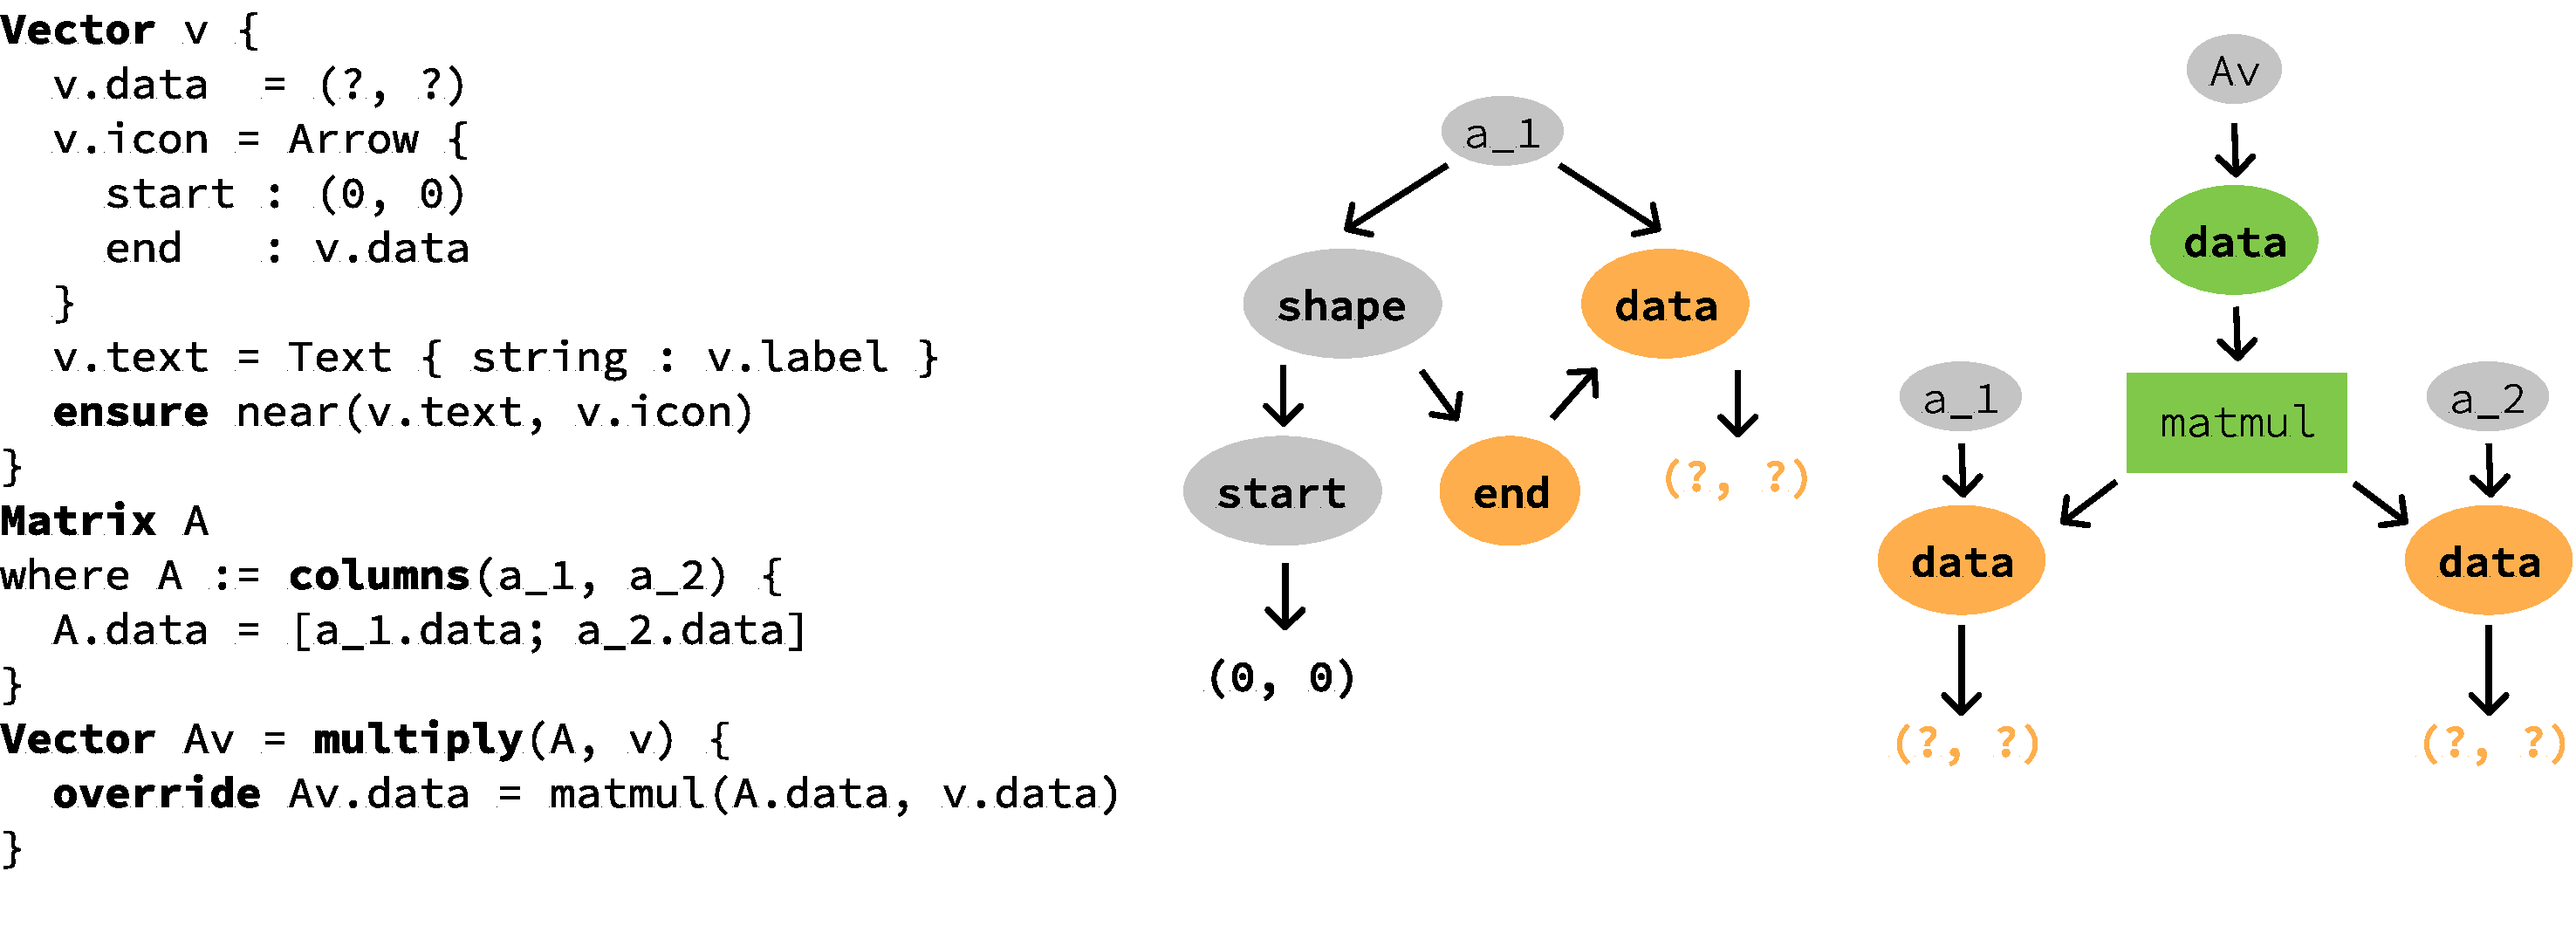
\includegraphics[width=\linewidth]{assets/chapter-4/eigen-comp-graph.pdf}
%     \vspace{-30pt}
%     \caption{\textbf{Left}: relevant blocks in the linear algebra \Style program for \cref{sec:ipenrose-example}. \textbf{Right}: computational graphs for \texttt{a\_1} and \texttt{Av}, where the \texttt{data} field for the former is optimized and that for the latter is computed.}
%     \label{fig:eigen-comp-graph}
% \end{figure}
% \vspace{10pt}

% Once exposed as draggable properties, the user can now change the values of positional DOFs by dragging shapes around. However, since their interaction is situated in an optimization problem, it's important to discuss how an optimizer influences this interaction and manipulates the rest of the diagram in a semantics-preserving way. In \cref{sec:ipenrose-example}, dragging \sty{a_1.icon.end} and \sty{a_2.icon.end} works as intended because they are independent from each other: they don't participate in the same constraints in the computational graph. However, this is not the right interaction for DOFs that participate in the same constraints, which is often the case. In this section, I give two example optimization strategies for supporting semantics-preserving drag.    
% \subsection{Follow the cursor}
% \label{sec:follow-the-cursor}

% \vspace{10pt}
% \begin{figure}[h]
%     \centering
%     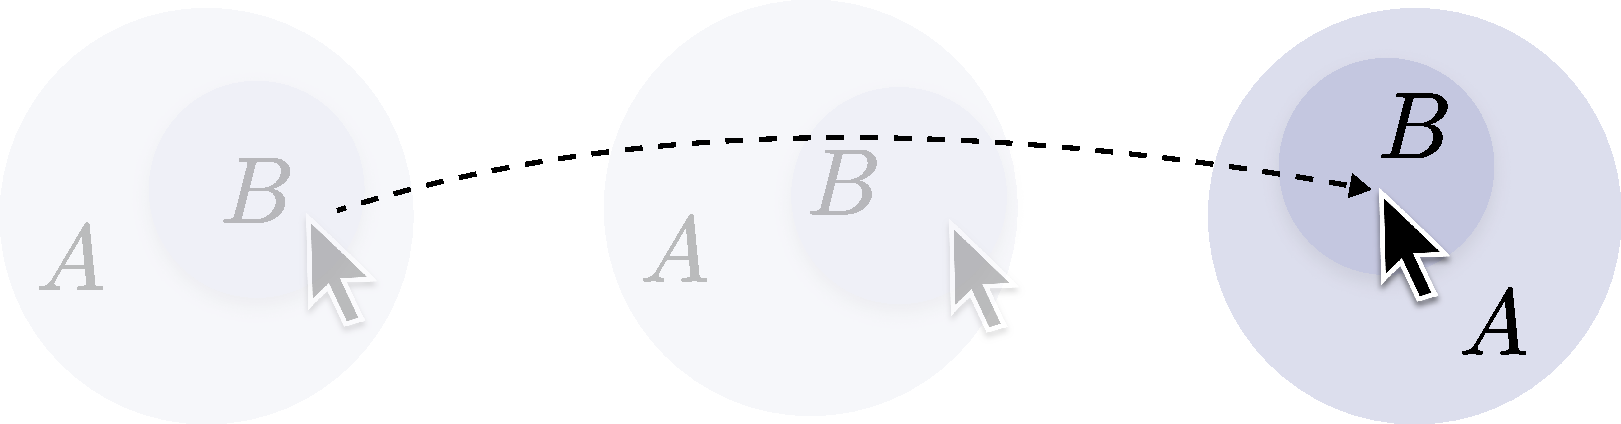
\includegraphics[width=0.8\linewidth]{assets/chapter-4/drag-expected.pdf}
%     \caption{Dragging a subset, $B$, in a Venn diagram in an intuitive and semantics-preserving way, where $B$ is always under the cursor and $B \subset A$ is always held true.}
%     \label{fig:drag-expected}
% \end{figure}
% \vspace{10pt}

% Consider the example in \cref{fig:drag-expected}, which shows a simple Venn diagram of sets $A$ and $B$ where $B \subset A$. The underlying rule of this visual representation is that a subset is always visually contained in the superset. An interactive diagram should clearly reveal this rule by keeping this containment relationship true at all times. For instance, if a student drags $B$ to the right, the diagram should change such that $A$ still contains $B$. Importantly, the interaction should be natural, and also make the feedback very clear: as the student is dragging $B$, $B$ must stay under the cursor, and the rest of the diagram should incrementally move with $B$ to maintain the containment relationship.

% Unfortunately, when using the current \Penrose optimizer, dragging either $A$ or $B$  yields counterintuitive results: the optimizer changes arbitrary properties, including the manipulated ones. This is because it optimizes all DOFs simultaneously. In \cref{fig:drag-default}, it moves both $A$ and $B$ to satisfy the containment constraint.  This behavior adds noise to the feedback, and may confuse the student.

% \vspace{10pt}
% \begin{figure}[h]
%     \centering
%     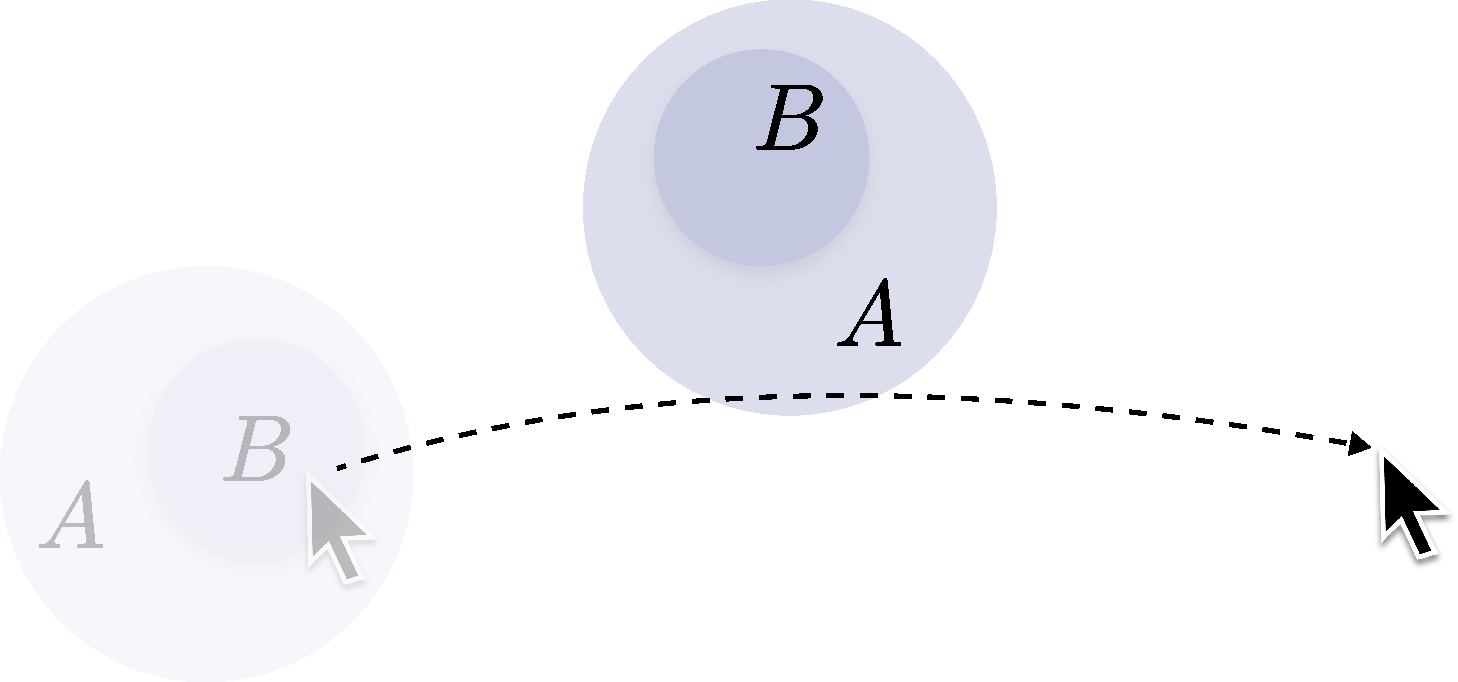
\includegraphics[width=0.75\linewidth]{assets/chapter-4/drag-default.pdf}
%     \caption{Dragging a subset, $B$, in a Venn diagram in semantics-preserving but counterintuitive way, where $B \subset A$ held true but the shapes appear in random locations.}
%     \label{fig:drag-default}
% \end{figure}
% \vspace{10pt}

% To enable intuitive interactivity, the system can analyze the computational graph again to derive the right behavior. We can achieve this behavior by ``locking'' the DOFs, treating them as constants in the optimizer. Specifically, when a student manipulates DOFs or its aliases, the system locks these DOFs and optimizes the rest as usual. When the student interacts with an object (\ie, dragging to change \sty{x} and \sty{y} of a \sty{Circle}), the system yields the control to the student completely and locks the manipulated properties during optimization. The visual effect is that all other parts of the diagram ``follow'' the student interaction. 

% \subsection{Freeze the world}
% \label{sec:freeze-the-world}

% Locking the manipulated property is not the only way to maintain the visual semantics. Instead of limiting the optimizer, we could also limit the interaction so they see the effect of changing one or multiple shape properties under constraints. When the student interacts with a shape, the optimizer keeps all other properties locked and continuously uses the energy function to “guide” the student. The techniques involved are different from \cref{sec:follow-the-cursor}. In this case, the student is playing the role of the optimizer, \ie, changing DOFs, while the optimizer only sends feedback to make sure the interaction is semantic. The visual effect is a constrained interaction where the student can only make semantically-valid moves. 

% \vspace{10pt}
% \begin{figure}[h]
%     \centering
%     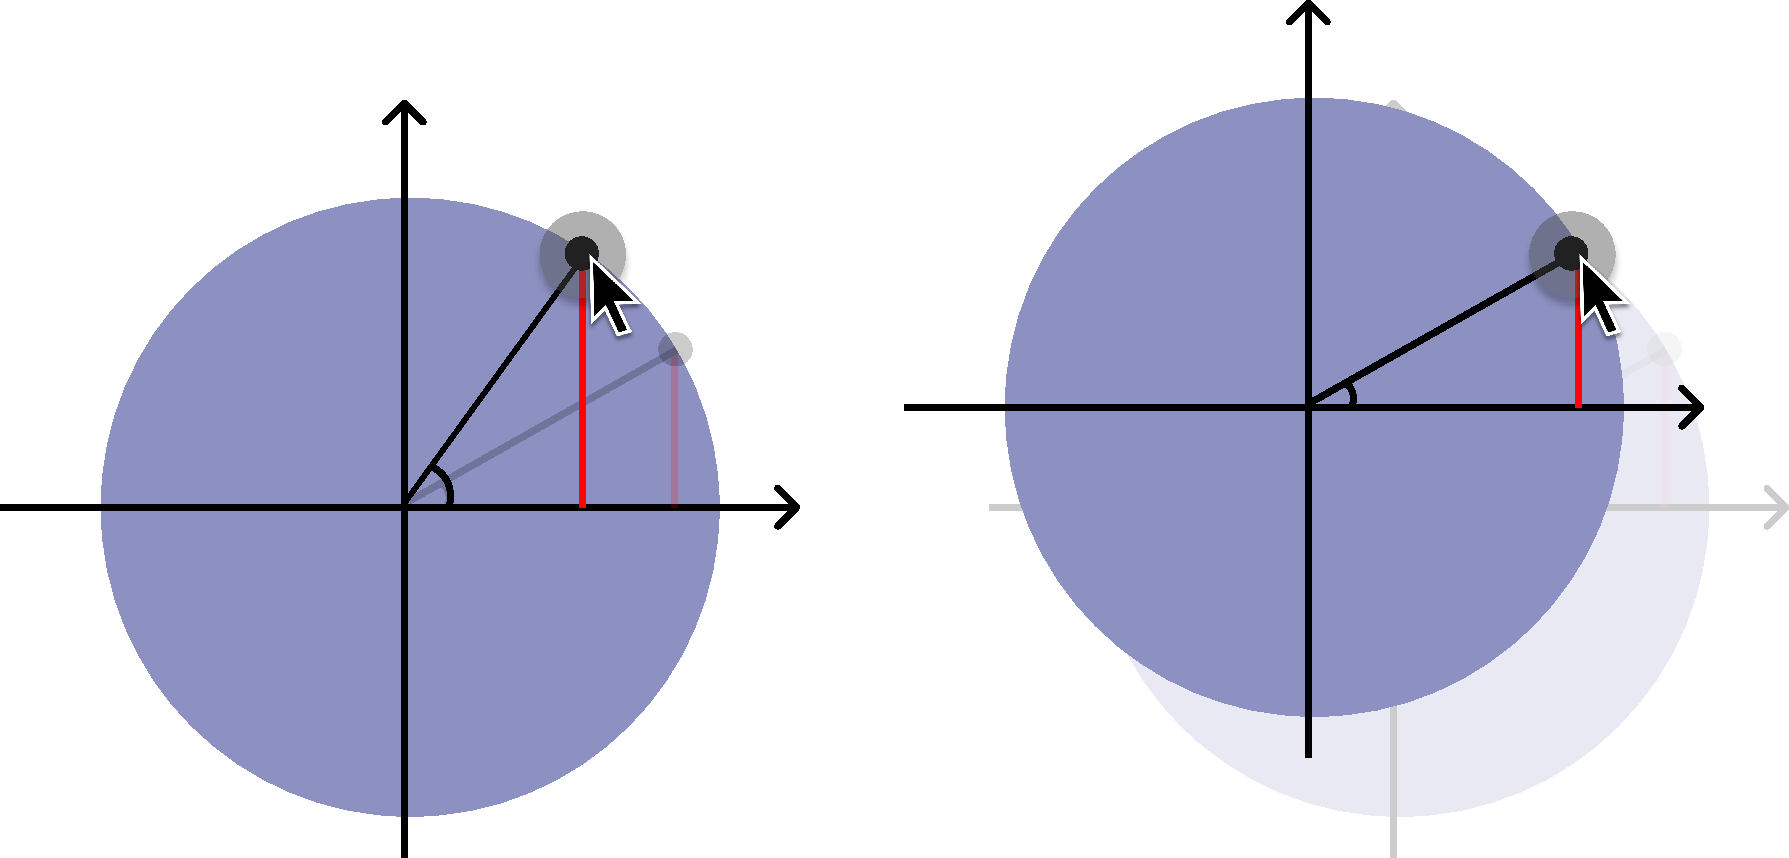
\includegraphics[width=0.75\linewidth]{assets/chapter-4/unit-circle-drag.pdf}
%     \caption{The behavior of dragging a point along the unit circle depends on the optimization strategy. \textbf{Left}: ``Follow the cursor'' shifts the entire diagram to follow the point and doesn't correspond to the mathematical semantics. \textbf{Right}: ``Freeze the world'' should be the correct optimization strategy, where the point only moves along the circle, and nothing else changes in the diagram.}
%     \label{fig:unit-circle-drag}
% \end{figure}
% \vspace{10pt}


% For instance, \cref{fig:unit-circle-drag} shows a diagram of the unit circle. A natural interaction is to drag the point along the unit circle to see how the values of trig functions change. In this case, the red line shows the value of $sin$. If the optimizer naively follows the cursor, \cref{fig:unit-circle-drag} (right) would be the result, where the rest of the diagram is translated to stay in a valid layout. Instead, it's much more desirable to ``freeze the world'' and constrain the student input within the feasible region—--along the unit circle (\cref{fig:unit-circle-drag} left).

% Together, these two strategies cover a wide range of drag behaviors that are traditionally difficult and time-consuming to implement. Note that these two strategies are not necessarily mutually exclusive. In fact, the system may have a set of default rules for or let the author specify the strategy on a per-DOF basis. For instance, an instructor might apply ``freeze the world'' to show students the valid positions of a component in a diagram, while applying ``follow the cursor'' to the rest of the components to show alternative layouts of the diagram. 


% \vspace{10pt}
% \noindent\textbf{Encoding optimization strategies.} If the author wants to control the optimization strategy, they will need an encoding to do so. Because \Style already has language constructs for matching on shapes, a \Style language extension may be suitable for specifying static strategies per shape, \eg, a shape should always follow the cursor when dragged. However, the current design of \Style may not be suitable for deciding strategies dynamically if needed, \eg, a shape follows the cursor in a certain region of the diagram, and freezes the world on the boundary. 
% \end{proposed}

% \section{Highlighting and annotation as feedback}
% \label{sec:highlight-and-annotate}

% \begin{proposed}

% As demonstrated in \cref{chp:edgeworth}, diagram understanding is a vital step towards representational fluency. A significant part of diagram understanding maps to learning the translational semantics of a diagram, \ie, which shape represents what math object. While \Edgeworth helps students practice the mapping between a particular visual representation and symbols, I propose to \textbf{provide on-demand, inter-representational feedback by utilizing the translational semantics of a \Penrose trio}. 

% \subsection{Inter-representational highlighting}

% Students' exposure to visual representations is often limited by traditional media like textbooks and in-person lectures. The mapping between symbolic and visual representations is often scarcely presented via prose, gesture, and carefully designed worked examples. Web-based materials show a much more pervasive use of on-demand highlighting to build up inter-representational connections. However, there’s also a non-trivial authoring burden to meticulously annotate the HTML document and the diagram with CSS classes:

% \vspace{10pt}
% \begin{figure}[h]
%     \centering
%     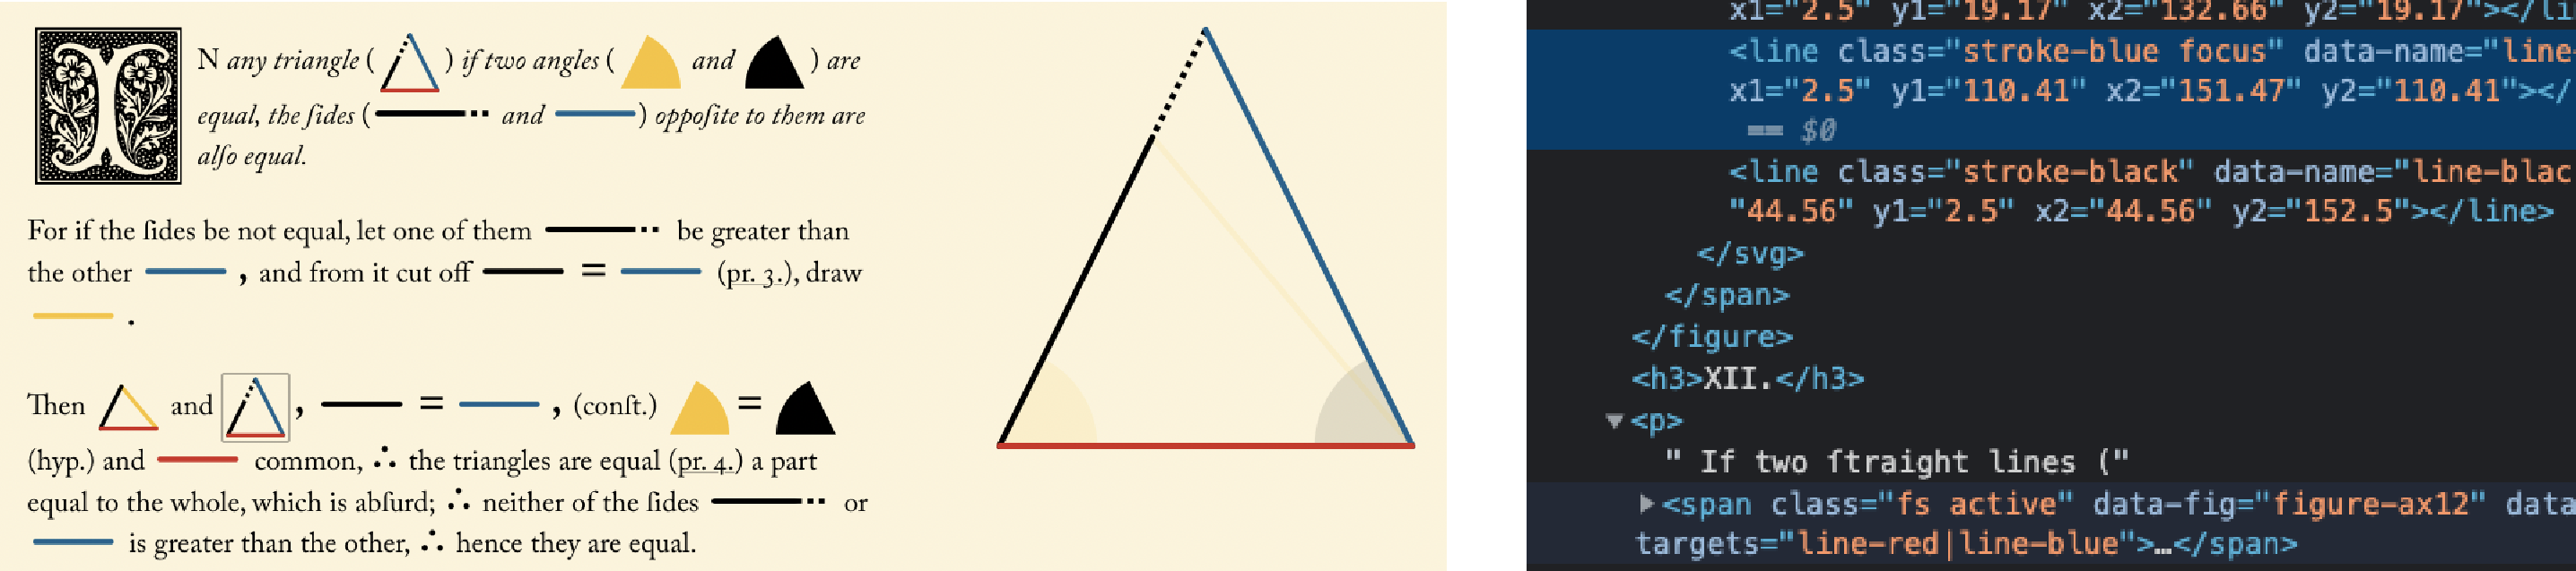
\includegraphics[width=\linewidth]{assets/chapter-4/euclid-highlight.pdf}
%     % \label{fig:euclid-highlight}
% \end{figure}
% \vspace{10pt}

% If an online textbook or website uses diagrams generated by \Penrose, the author may leverage the translational semantics to automatically provide on-demand highlights. For instance, suppose an author writes an visual explanation in markdown with interleaving \Substance symbols in the prose. The system can automatically generate diagrams by extracting the \Substance symbols and provide highlights for all subsequent references to the same symbols. Since \Penrose can generate alternative diagrams in the same visual presentations, the highlighting can also provide contrasting cases of a particular entity across diagram instances.

% \vspace{10pt}
% \begin{figure}[h]
%     \centering
%     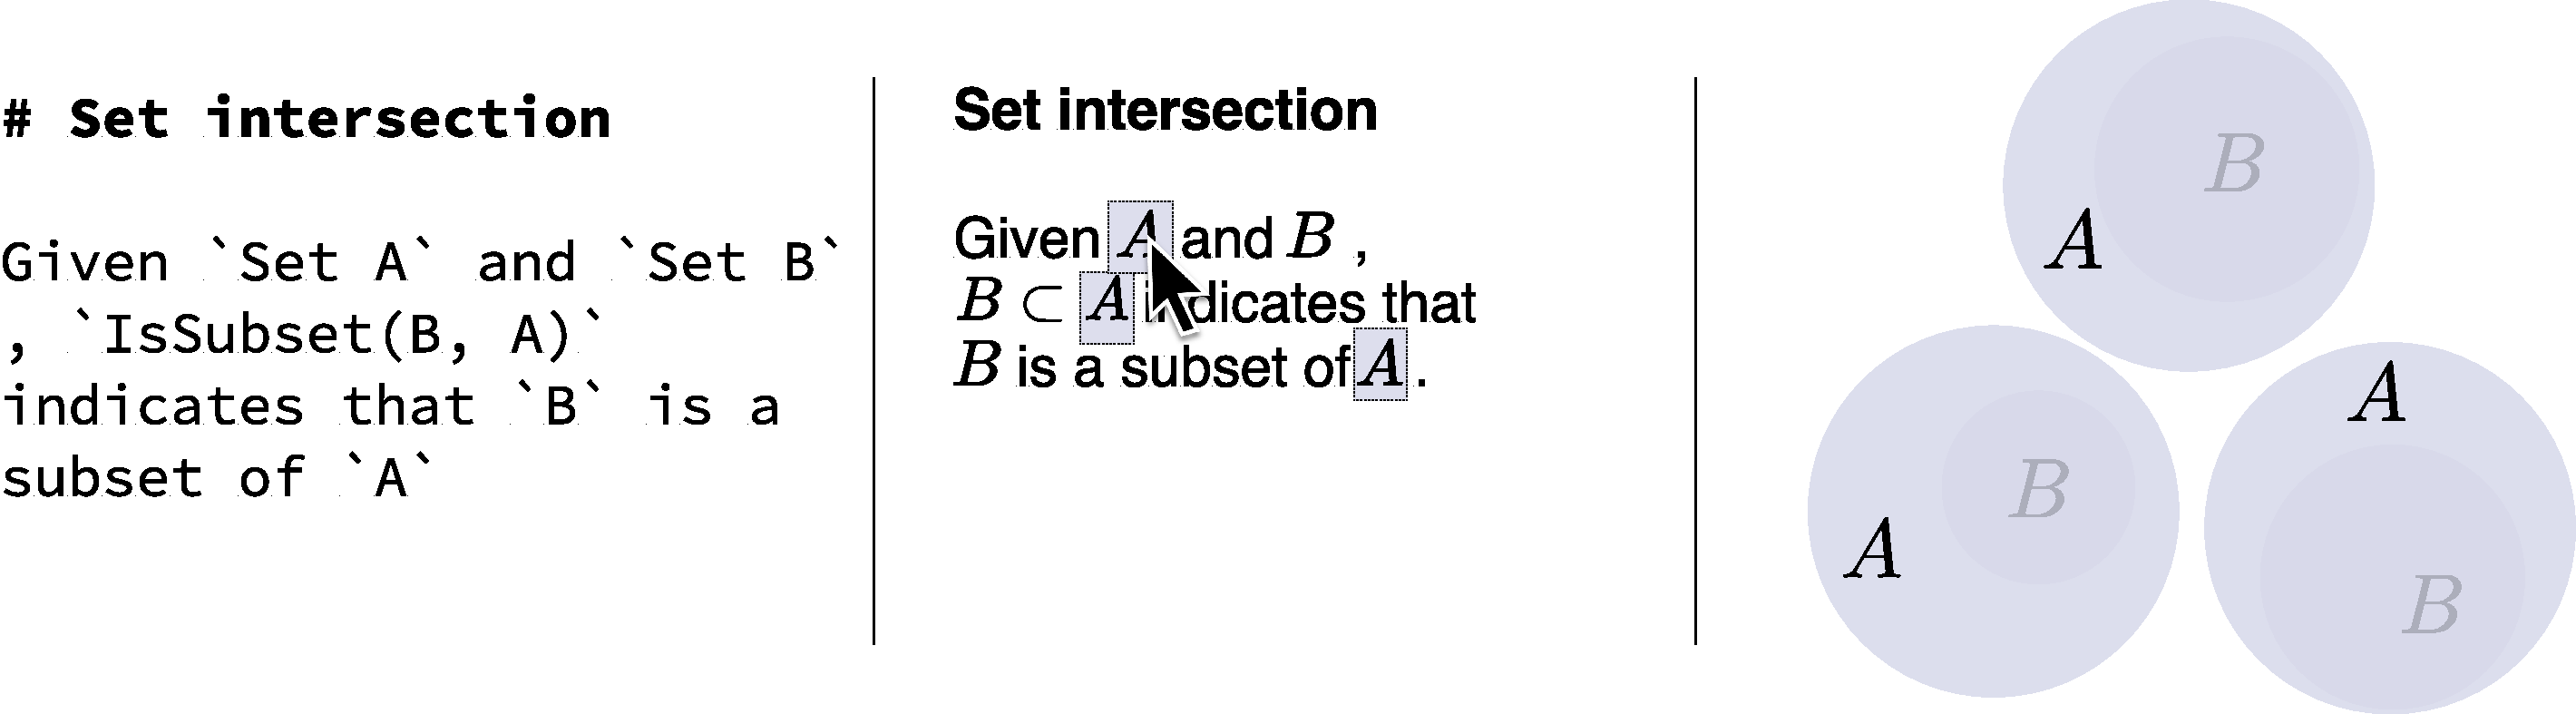
\includegraphics[width=\linewidth]{assets/chapter-4/markup-highlight.pdf}
% \end{figure}
% \vspace{10pt}

% Building connections among multiple visual representations also improve learning~\cite{multipleReps}. Because a \Penrose trio is representationally salient, one can swap among alternative \Style programs to get diagrams that visualize the same symbols. Because the \Substance program stays the same, the same strategy also works for highlighting diagram parts across multiple visual representations.

% \vspace{10pt}
% \begin{figure}[h]
%     \centering
%     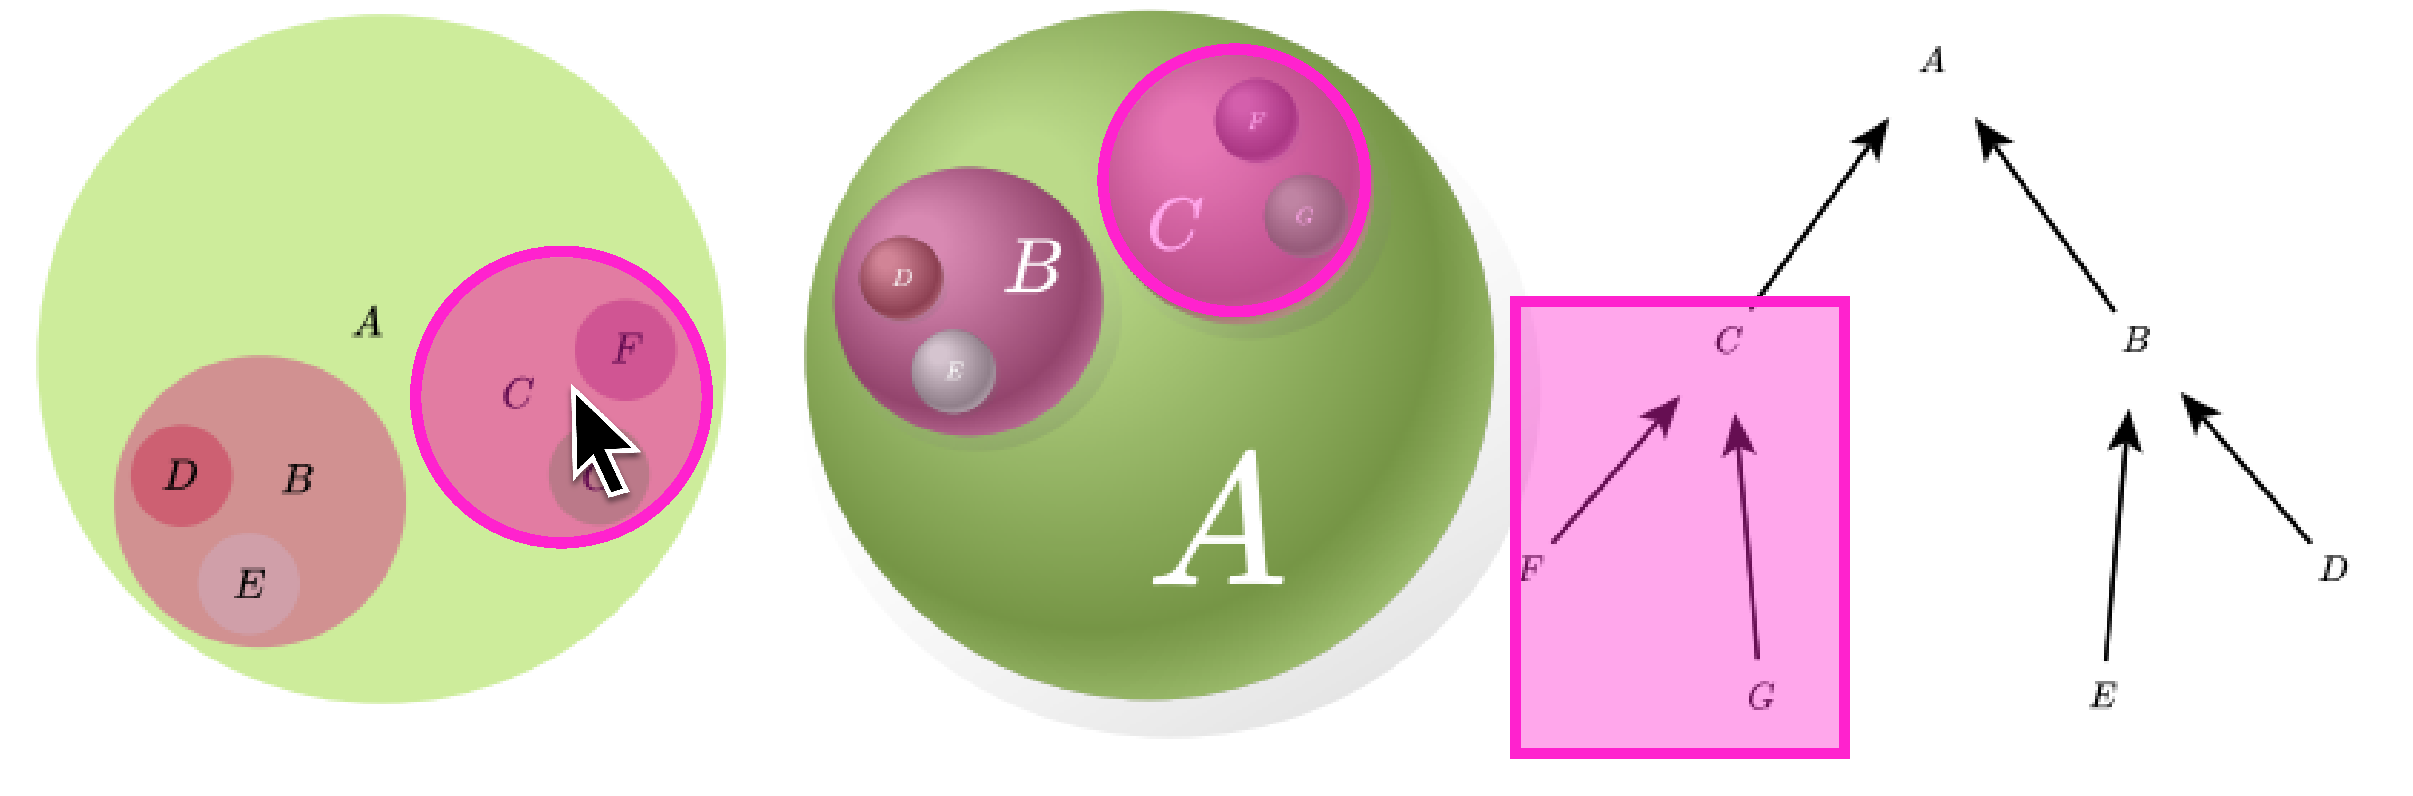
\includegraphics[width=0.9\linewidth]{assets/chapter-4/multirep-highlight.pdf}
% \end{figure}
% \vspace{10pt}

% \subsection{Documentation and program slices as tooltips} 

% \vspace{10pt}
% \begin{figure}[h]
%     \centering
%     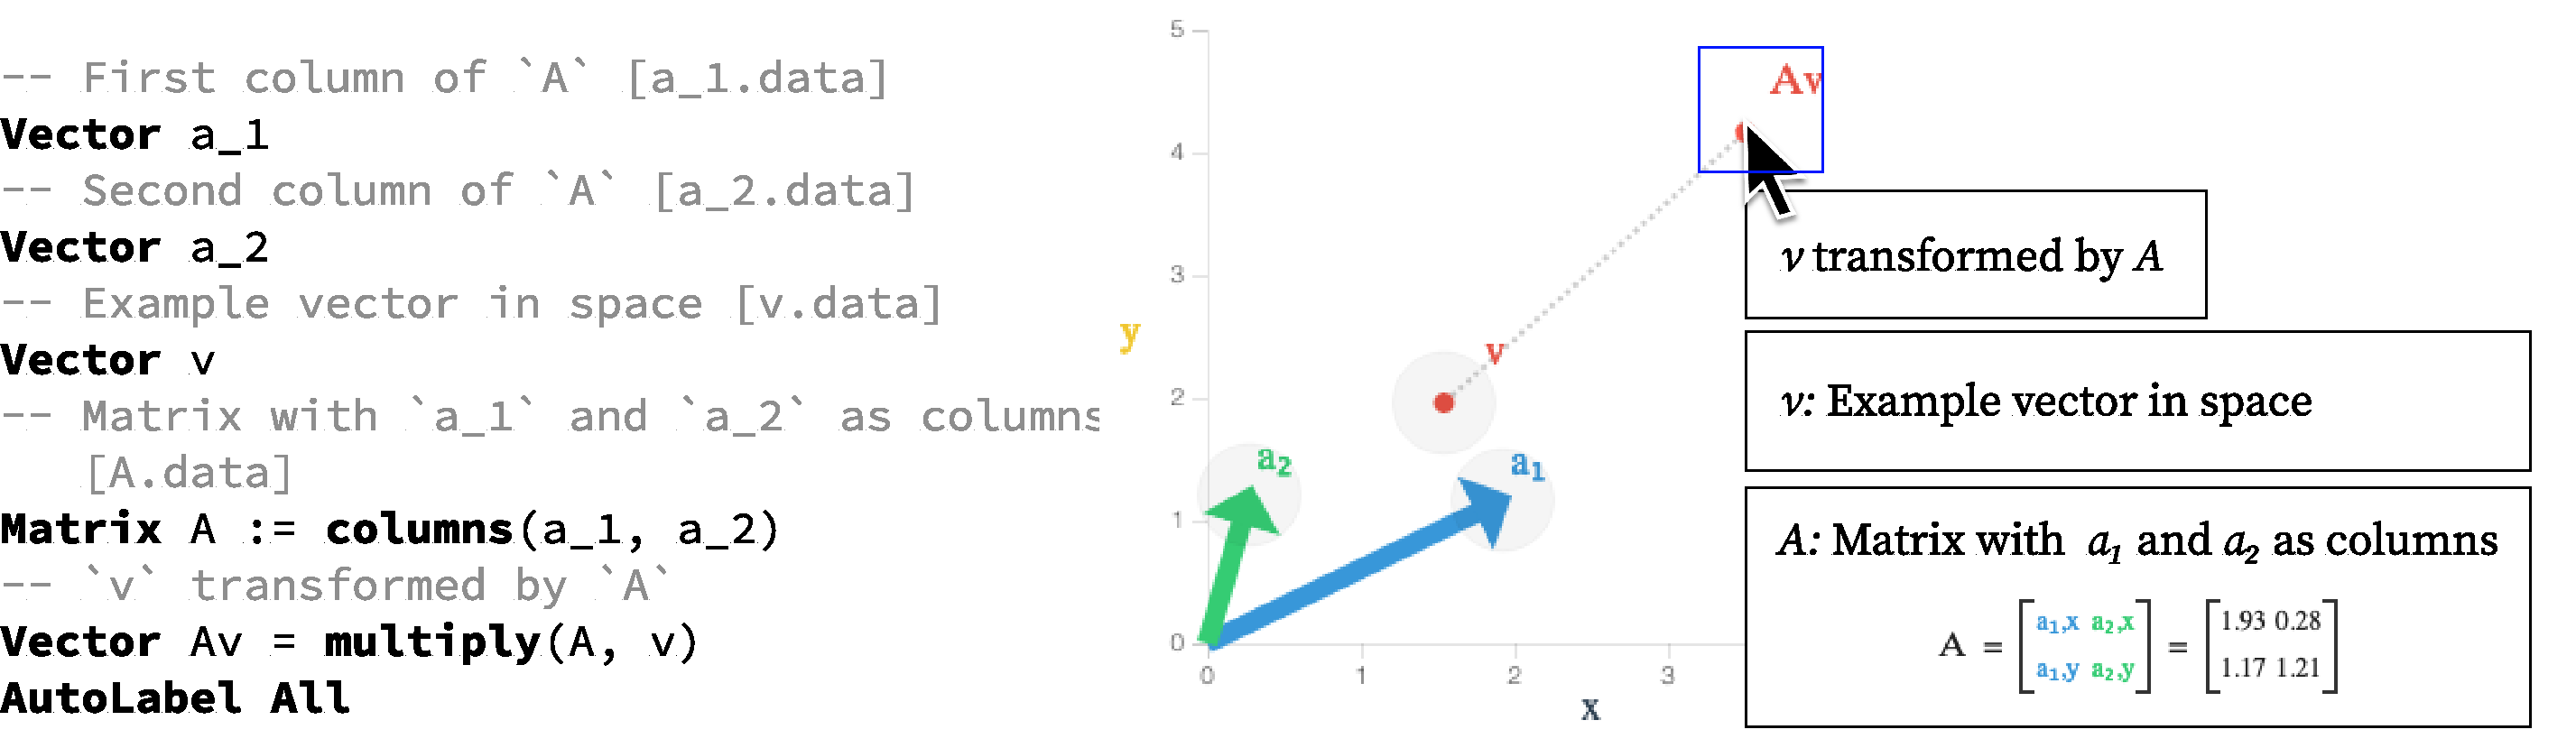
\includegraphics[width=\linewidth]{assets/chapter-4/docs-tooltips.pdf}
% \end{figure}
% \vspace{10pt}

% In technical documents, symbols and acronyms are often defined once and used everywhere else. To help readers understand them, tools like ScholarPhi and Nota~\cite{scholarPhi, nota} use tooltips to aid readers. In real world publications, authors augment math equations for better readability, too. Diagrams use even more symbolism and can be hard to understand. We propose a lightweight markup language in the form of \Substance documentation for authoring simple \emph{diagram augmentation}. Similar to Idyll~\cite{idyll}, the markup language has a markdown-like syntax, but allows splices of \Substance variables and runtime values. In the frontend, we analyze the \Substance values in each snippet, and trace all related snippets based on variable references. For instance, the snippet about $Av$ refers to both $A$ and $v$, so they appear on the tooltip stack.

% The translational semantics also involve how \Domain, \Substance, and \Style programs relate to each other. Therefore, \Style and \Domain can also be valuable sources of feedback: the \Style program encodes the visual semantics, and the \Domain program captures the grammar of notations. A slice of a \Penrose trio traces the origin of a graphical primitive to the \Domain, \Substance, \Style programs. For instance, without any authoring burden, the system can display slices of the program trio based on object selection. Alternatively, the proposed markup language may be extended to \Domain and \Style, and the system can render inline documentations in all three languages.

% \vspace{10pt}
% \begin{figure}[h]
%     \centering
%     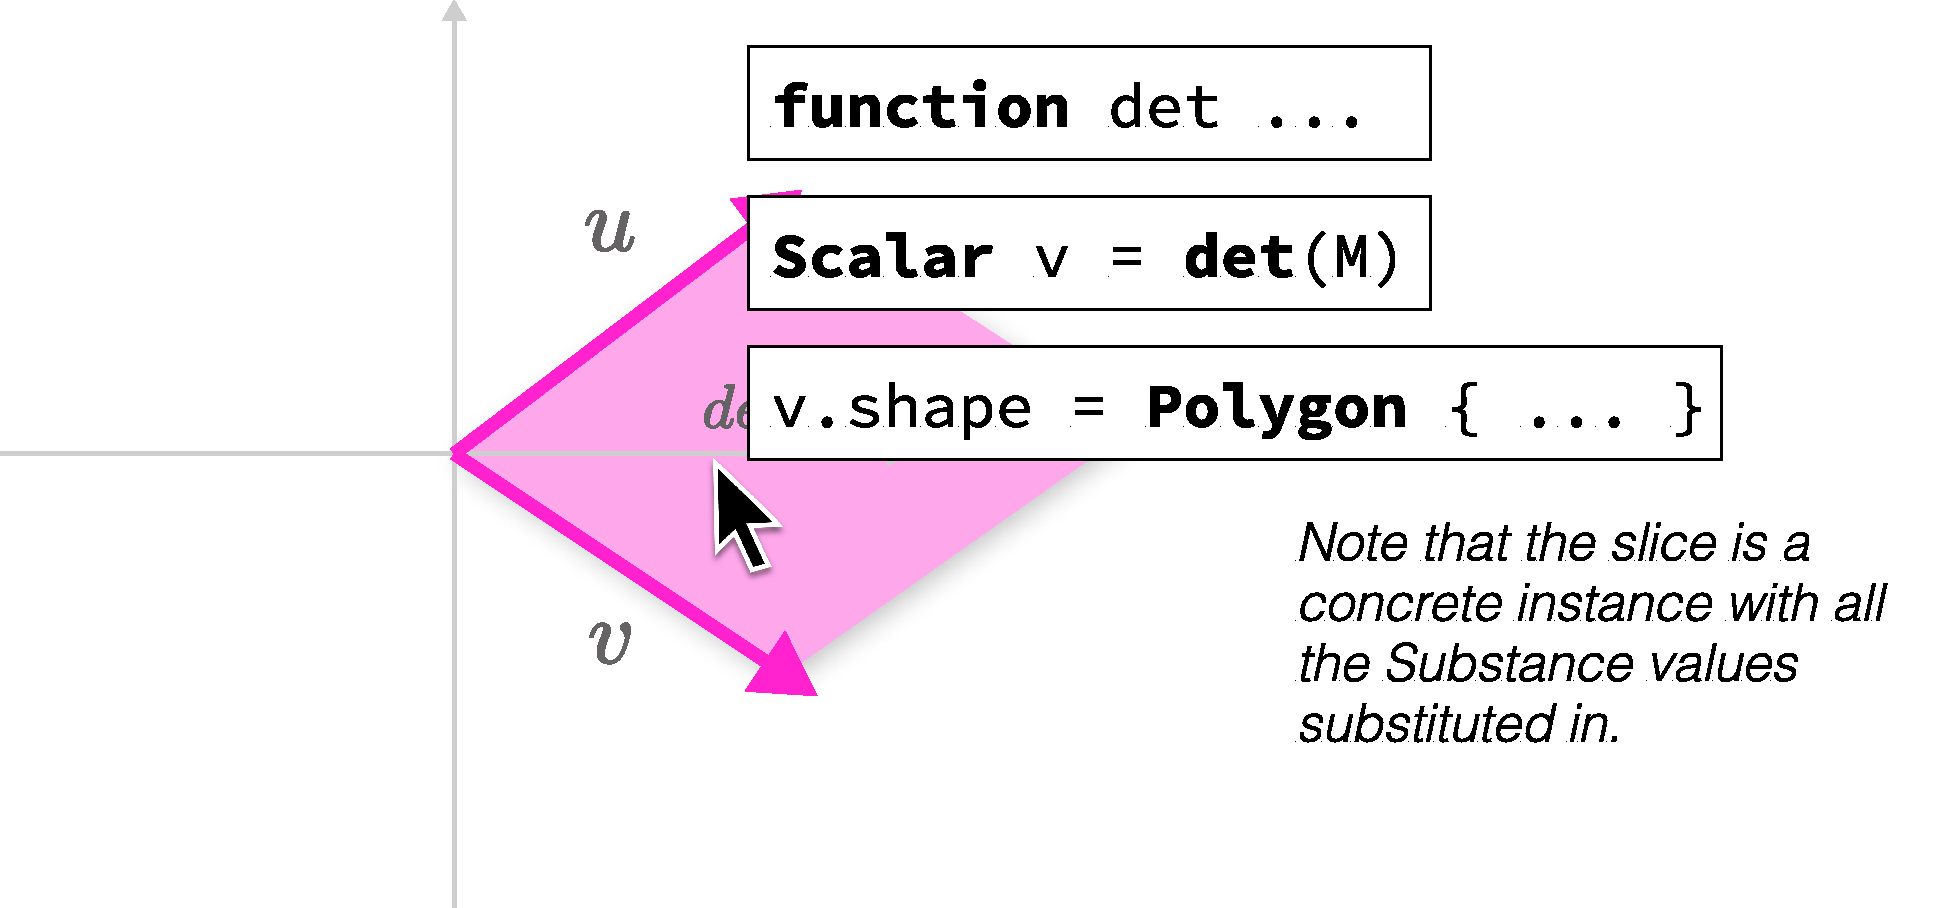
\includegraphics[width=0.75\linewidth]{assets/chapter-4/slices.pdf}
% \end{figure}
% \vspace{10pt}
% \end{proposed}

% \section{Evaluation}

% \begin{proposed}
% To evaluate the discussed interactive techniques, I plan to conduct comparative case studies between feature-full modern JavaScript libraries (e.g. D3.js) and \Penrose. Research questions for this study include:
% \begin{itemize}
%     \item Does the \Penrose-based system simply programming interactive diagrams?
%     \item Are the interactive features comparable to the hand-written examples? 
%     \item How expressive is our grammar of interactivity?
%     \item When does the approach break down?
% \end{itemize}

% In general, I expect that our system can cover common, important interactive features with significantly less manual effort. In the studies, I plan to collect both quantitative (\eg, lines-of-code, time taken) and qualitative data about authoring interactive diagrams using JS library versus our system. Currently, the candidate pool of examples include:

% \begin{itemize}
% \item Worked examples and explorable explanations:
%     \begin{itemize}
%         \item A Gentle Introduction to Graph Neural Networks: \url{https://distill.pub/2021/gnn-intro/}
%         \item Explained visually: \url{https://setosa.io/ev/}
%         \item Explorable explanations: \url{https://explorabl.es/}
%         \item Gallery of concept visualization: \url{https://conceptviz.github.io/}
%     \end{itemize}
% \item Online textbooks and curricula:
%     \begin{itemize}
%         \item Seeing theory: \url{https://seeing-theory.brown.edu/}
%         \item Immersive math: \url{http://immersivemath.com/ila/index.html}
%         \item Mathigon: \url{https://mathigon.org/}
%         \item Physically-based rendering: \url{https://pbr-book.org/}
%         \item Brilliant: \url{https://brilliant.org/}
%     \end{itemize}
% \end{itemize}
% \end{proposed}

\section{Concluding remarks}

Curiously, building authoring tools for rich, interactive diagrams, narratives, and learning activities seems just the right amount of material for a second dissertation,\footnote{In the spirit of \citet{barik_error_nodate}} or a full-time job.